\chapter{CloudVision环境建设及实验验证}
\label{cha:cloudvision_experiment}
本章描述基于OpenStack建设的私有云,用于做CloudVision的实验和学院老师及同学。
在章\ref{sec:priv-cloud-deployment}我们描述规划和部署私有云的细节,了解到
CloudVision实验的环境情况。
为了了解CloudVision架构的特性,我们做了两个实验,横向扩展性实验和内存缓存实验。
在章\ref{sec:scalability-experiment}描述做的横向扩展性实验,了解到在增加
计算节点的情况下是否能提高性能。在章\ref{sec:memory-cache-experiment}描述
做的内存缓存实验,了解到内存缓存在不同机器视觉库应用带来的性能提高。


\section{OpenStack私有云实验环境建设}
\label{sec:priv-cloud-deployment}
为了给学院的老师与同学提供一个灵活的基础设施环境,我们建设的
清华软件学院的信息系统与工程研究所多租户的OpenStack私有云。
目前已经有多个用户同时在使用建设的私有云。在2014年秋天开的
叶晓俊老师开的云数据管理(1),用到了建设的私有云,给课程的
学生提供实验环境,每个组分配了3个服务器,总共有7个组,
用到了21个虚拟机。通过OpenStack可以快速提供立即能用到
的服务器资源,用完了回收给资源迟,提供给别人用。所以
特别合适于给课程的学生用,提供灵活的基础设施。
在OpenStack之前,课程的学生得在自己电脑装虚拟机或者
去机房手动部署操作系统等等才能做实验,建立的私有云
提基础设施的使用率和实验效率。

另外实验室里的同学也用到了建设的私有云提供研究和实验环境。
丁贵广几个研究项目,本论文的CloudVision开,Hadoop自动部署,MongoDB研究,用到
私有云提供开发和实验环境。CloudVision的横向扩展性实验和内存缓存实验,
用了私有云提供的服务器资源跑实验,另外用了OpenStack Swift的对象存储
保存实验的数据集和结果。

\subsection{私有云部署规划}
这里我们描述建设的过程和细节。建设流程分了三个阶段:
先设计与规划需要的硬件资源和分配角色,然后基于准备准备的方案准备硬件和部署OpenStack,
最终基于功能测试保证可用性和提供平台的技术支持。

我们部署了OpenStack的Juno版本。每个OpenStack组件都得选使用什么技术去实现。我们选了Nova组建使用KVM,
选了Neutron使用OVS + VLAN实现网络服务,
选了Cinder,Swift和Nova零时存储使用分布式的Ceph存储提供统一化的存储实现。
另外我们使用了Fuel部署和管理OpenStack平台本身。
在OpenStack环境的部署分成不同的角色:Controller(控制节点),Compute(计算节点),Storage(存储节点),Fuel Master(部署节点)。
Controller是主要跑OpenStack的API,界面,数据库,信息队列,调度器。Compute是
负责跑虚拟机。Storage节点是执行Ceph的软件提供高可用的存储集群。
每个角色硬件需求不一样,Controller需要少量的CPU,内存和磁盘,
Compute主要需要CPU和内存,Storage主要需要磁盘。

为了不浪费资源,我们用到了学院原有的服务器,总共学院提供了
7台物理服务器,在表\ref{tab:hardware-table}可以看到
每个服务器具体的配置和分配的角色。第一个服务器ctrl1-2-mix
为了更好的利用到有限的资源使用三个KVM虚拟机跑
两个Controller节点和一个Fuel的节点。另外选了使用Compute和Storage
的混合角色,原因同样为了更好的利用资源。
\begin{table}[H]
  \centering
  \begin{minipage}[t]{0.98\linewidth} % 如果想在表格中使用脚注,minipage是个不错的办法
  \caption[私有云硬件配置和分配]{私有云硬件配置和分配}
  \label{tab:hardware-table}
    \begin{tabularx}{\linewidth}{lXlX}
      \toprule[1.5pt]
        名字 & 牌子和配置 &  物理位子 & 注解\\
        ctrl1-2-mix & 自己组装\newline(24CPU, 80GB, 4x1.8TB) & r1n2 & Fuel, Controller1, Controller2  \\
        ctrl3-ceph & 自己组装\newline(24CPU, 64GB, 4x1.8TB) & r1n5 & Controller和Storage角色  \\
        compute1 & 自己组装\newline(24CPU, 56GB, 4x1.8TB) & r1n3 & Compute和Storage角色  \\
        compute2 & 自己组装\newline(24CPU, 80GB, 4x1.8TB) & r1n1 & Compute和Storage角色  \\
        compute3 & 自己组装\newline(24CPU, 64GB, 4x1.8TB) & r1n4 & Compute和Storage角色  \\
        compute4 & Dell PowerEdge R910\newline(48CPU, 64GB, 3x0.5TB) & r1n7 & Compute和Storage角色  \\
        compute5 & Dell PowerEdge R910\newline(48CPU, 64GB, 3x0.5TB) & r2n7 & Compute和Storage角色  \\
      \bottomrule[1.5pt]
    \end{tabularx}
  \end{minipage}
\end{table}


\subsection{私有云网络方案}
在OpenStack的部署,最容易出问题和规划是网络部分,主要原因是OpenStack也提供网络虚拟化同时
OpenStack自己的网络架构复杂。这里我们简单描述OpenStack的网络,具体网络规划,物理和逻辑网络拓扑。

\begin{figure}[h]
  \centering
    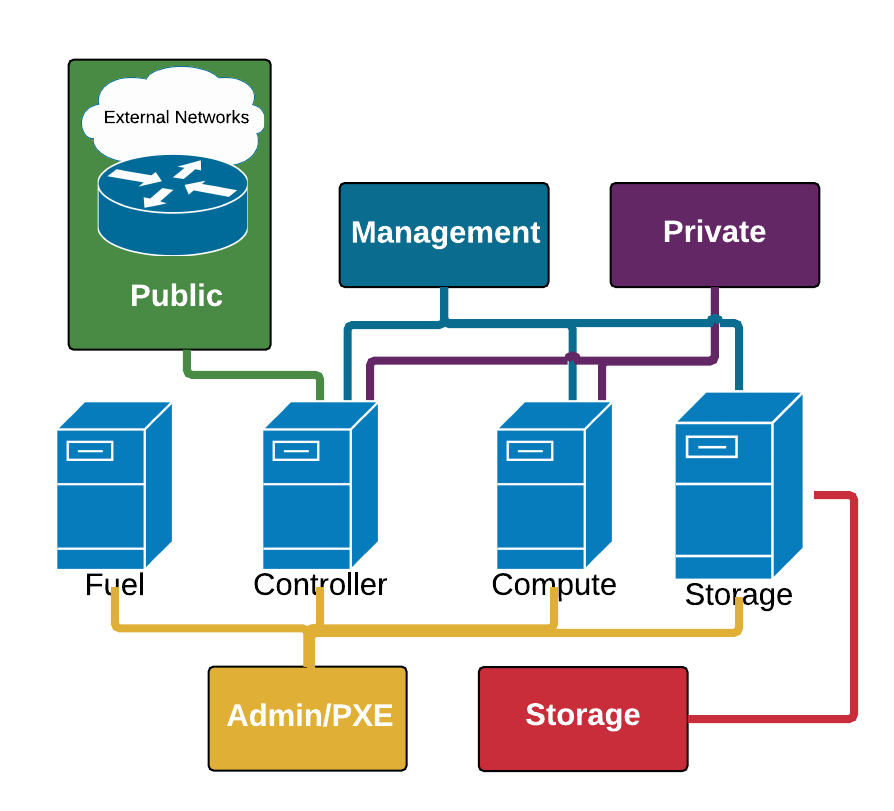
\includegraphics[width=0.50\textwidth]{os-logical-networks}
  \caption{OpenStack逻辑网络拓扑}
  \label{fig:os-logical-networks}
\end{figure}
在图\ref{fig:os-logical-networks}可以看到我们的OpenStack逻辑网络拓扑。
图里分成不同的角色,将每个角色描述清楚它属于哪些网络。我们定义了五种网络:
Public/Floating(对外网络),Management(OpenStack本身管理网络),Private(虚拟机私有网络或者租户网络),
Admin/PXE(部署网络)。Public/Floating网络负责给虚拟机和OpenStack本身提供对外访问接入,因此需要跟OpenStack外面的路由器
集成,比如在企业内部
的所有员工能访问的网络或者校园网络是一个Public网络,只有Controller节点需要在Public网络宣传出去。
Managent网络负责OpenStack集群内部的消息传输,所以Controller,Compute和Storage都需要在
这个网络。Private用于虚拟机之间(私有网络)的流量,比如在不同的计算节点的虚拟机通信,所以Controller和
Compute在Private网络里,Controller有一个虚拟路由器负责路由Private到Public的流量。Storage网络用于
存储节点内部的分布式存储副本复制流量,只有Storage节点在这个网络里。Admin/PXE的网络限于部署操作系统
和配置软件用,所有节点都需要在这个网络里面。分开各个网络为了考虑到安全和性能的需求,比如计算节点为了安全考虑
不能直接从外面被访问,那如果只用一个网络就无法做这样的隔离,另外Storage网络对网络IO要求很高如果把他单独分开,可以
将Storage网络放在高IO的网卡。

在表\ref{tab:network-table}描述我们每个逻辑网络分配了什么VLAN和IP和相应的服务器网卡,通过例子可以荣理解
网络的关系。表里的Tagged表示在服务器的网卡通过操作系统的支持打VLAN标,Native表示服务器的
网卡不打VLAN标签但是包到交换机会打VLAN标签。每个服务器物理网卡只能有一个Native VLAN但是可以
有多个Tagged VLANs,通过Tagged VLANs可以分配多个逻辑网络到一个网卡。
Public使用白老师给我们分配的校园IP段和网关,其他网络都自己分配了RFC1918的私有网段。
\begin{table}[h]
  \centering
  \begin{minipage}[t]{0.98\linewidth} % 如果想在表格中使用脚注,minipage是个不错的办法
  \caption[私有云网络VLAN和IP分配]{私有云网络VLAN和IP分配}
  \label{tab:network-table}
    \begin{tabularx}{\linewidth}{lXXX}
      \toprule[1.5pt]
        名字 & vlan &  IP段 & 物理网卡\\
        Public & 102 (Tagged)  & 166.111.80.16/28\newline GW: 166.111.80.10 & Eth1  \\
        Management & 100 (Tagged)  & 192.168.150.0/24 & Eth1  \\
        Private & 1000-1300 (Tagged) & 租户自己定义 & Eth1  \\
        Storage & 101 (Tagged) & 192.168.151.0/24 & Eth0  \\
        Admin/PXE & 105 (Native) & 10.20.0.20/24 & Eth0  \\
      \bottomrule[1.5pt]
    \end{tabularx}
  \end{minipage}
\end{table}

难点在于交换机需要特殊配置,每个交换机到服务器的口是一个Trunk口,允许服务器自己打VLAN标签。
在表\ref{tab:network-table},可以看到我们用到了两个物理网卡,都是需要连到交换机,但是配置不一样。
Eth0需要练到一个交换机一个Trunk口,配成允许101(Tagged)和Native VLAN 105。
Eth1需要练到一个交换机一个Trunk口,配成允许100,102,1000-1300(Tagged)。
学院提供了一台神州数码DCS-4500-26T交换机,有24个千兆口。因为Eth0和Eth1连到交换机的配置不一样,
需要固定交换机的口,为了容易分别Eth0和Eth1的口我们把交换机分成两块,交换机口1到12属于eth0,
交换机口13-24属于eth1。另外环境也需要跟校园网络集成,所以我们划分了一个交换机口,接入校园网络同时
在校园网络打VLAN 102标签。在表\ref{tab:network-switch}可以看相应的交换机的配置。

\begin{table}[h]
  \centering
  \begin{minipage}[t]{0.78\linewidth} % 如果想在表格中使用脚注,minipage是个不错的办法
  \caption[私有云网络神舟数码交换机配置]{私有云网络神州数码交换机配置}
  \label{tab:network-switch}
    \begin{tabularx}{\linewidth}{lXXX}
      \toprule[1.5pt]
        交换机口 &   配置 \\
        1-12 (Eth0) & switchport mode trunk\newline switchport trunk native vlan 105\newline switchport trunk allowed vlan 101  \\
        13-24(Eth1) &  switchport mode trunk\newline switchport trunk allowed vlan 100,102;1000-1300 \\
        26(校园介入) & switchport access vlan 102  \\
      \bottomrule[1.5pt]
    \end{tabularx}
  \end{minipage}
\end{table}

\subsection{私有云总结}
我们部署了一个7台服务器的OpenStack环境,详细描述了部署过程和细节,使可能别人重用我们的部署经验。
我们的私有云环境也有活跃的用户,需要为他们维护部署的OpenStack环境,保证平台可用。在
维护中我们也碰到了问题和修复问题,包含物理硬盘损坏,网线松了,Ceph卡死,等等。虽然有问题,
我们还是认为OpenStack减少所有用户总体的维护成本。




\section{横向扩展性实验}
\label{sec:scalability-experiment}
这个实验的目标是了解到CloudVision云平台不同功能的扩展性。通过增加业务与处理层的计算节点,
应该能看到一个线性的运行时间的减少。本实验使用了Caltech-256的数据集,里面
有30607图片和256个类别,总体数据大小是1.2GB。

扩展性实验分析\ref{subsec:sift-scalability} SIFT特征抽取扩展性和\ref{subsec:bow-learning-scalability}
BoW字典学习扩展性。两个实验同样从1台计算节点增加到4台计算节点,分析计算时间。
每台计算服务器使用m1.large的配置,8 x 2.4Ghz vCPU,16GB内存,160GB本地硬盘。所有虚拟机共享一个
1Gbps私有网络。

\subsection{SIFT特征抽取扩展性实验}
\label{subsec:sift-scalability}
这个实验分析CloudVision实现的分布式SIFT特征抽取扩展性能力。
首先为实验把Caltech-256的数据集做成一个1.2G的SequenceFile保存
到OpenStack Swift对象存储。然后执行在\ref{sec:feature-extraction}描述CloudVision SIFT特征抽取实现,
保存SIFT特征到OpenStack Swift。

测量方法是在业务与处理集群,直接在Mesos Master通过Linux命令
提交Spark的任务,因为本实验不想考虑控制层的影响。
我们测量Spark的SIFT特征抽取任务的计算时间,从提交Spark任务
开始测量,Spark任务结束了停止时间测量。计算时间包括Spark和Mesos
的调度和启动时间。

\begin{figure}[h]
  \captionsetup[subfigure]{aboveskip=2pt,belowskip=2pt}
  \centering
  \begin{subfigure}[b]{0.49\textwidth}
    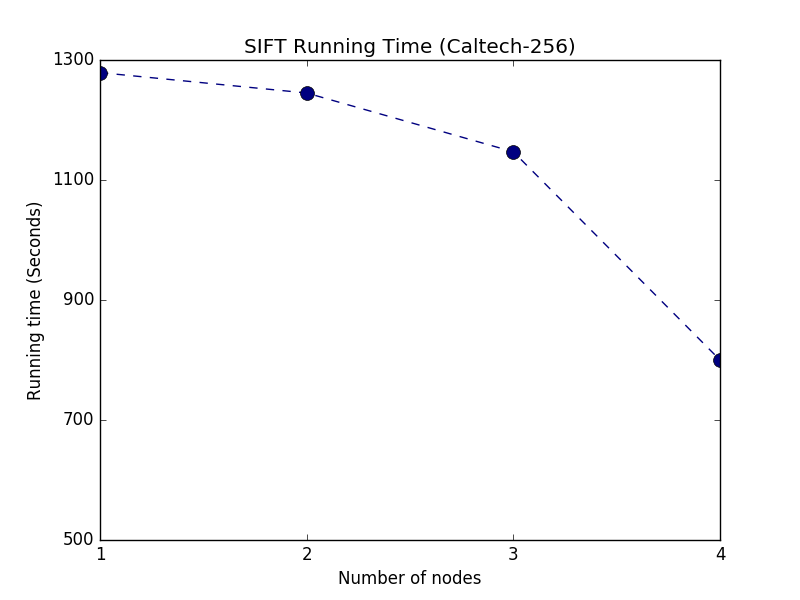
\includegraphics[width=\textwidth]{sift_running_time}
    \caption{Caltech-256数据集}
    \label{fig:sift-running-time}
  \end{subfigure}
  \begin{subfigure}[b]{0.49\textwidth}
    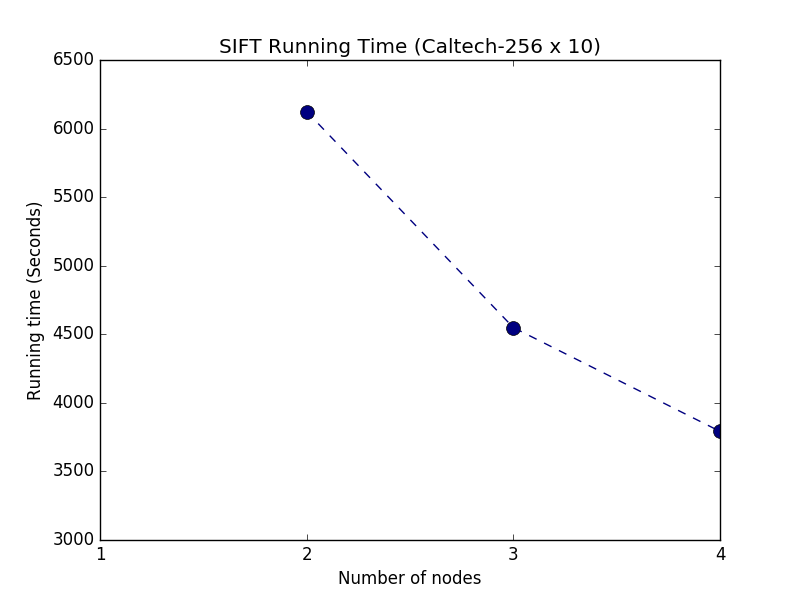
\includegraphics[width=\textwidth]{sift_running_time_10x}
    \caption{10倍的Caltech-256数据集}
    \label{fig:sift-running-time-10x}
  \end{subfigure}
  \caption{SIFT特征抽取计算时间}

\end{figure}

在图\ref{fig:sift-running-time}可以看到在增加Spark计算计算节点情况下,
SIFT特征抽取任务计算时间的变化。从图可以看到增加计算节点能提高性能,
但是增加节点时候提高的性能不高。在用一个计算节点的时候使用了1279秒
执行完任务,增加到两个计算点时候使用了1245秒,增加到
三个计算节点使用了1147秒,最后增加到四个节点使用了800秒。
这个提高性能的量是不理想,增加节点基能线性减少计算时间。
假设$n$表示计算节点数量,$t_n$表示用$n$个节点的计算时间,
$o$表示任务开销时间,
那理想的$t_n$运算时间为定义
\begin{equation} \label{eq:running-time}
t_n = \frac{t_1}{n} + o
\end{equation}
理想情况公式里$o$开销时间尽量少。
在图\ref{fig:sift-running-time},可以看到没有达到理想的情况,
我们认为Spark的任务
开销和写到Swift的Disk I/O造成$o$太大。

为了了解到为什么计算时间在增加
计算节点的时候没有按照在\ref{eq:running-time}定义的理想公式减少,
我们重新执行了本次实验但是数据集比原来数据集大10倍。我们写了一个脚本
复制Caltech-256的图像10次,将10倍大小的Caltech-256数据集做成一个
SequenceFile上传到Swift,Caltech-256的SequenceFile大小是12GB。
除了数据集大小其他参数和算法跟在图\ref{fig:sift-running-time}执行的实验一样,
在图\ref{fig:sift-running-time-10x}可以看到在10倍大小Caltech-256数据集的跑实验的结果。
跑实验过程中用一个计算节点的时候实验无法执行完成,因为Spark开始出Out of Memory异常,
所以用一个计算节点没有记录数据。
增加到两个计算节点使用了6124秒执行完成实验,增加到三个计算节点使用了4549秒,增加到四个计算节点使用了3729秒。
我们认为在更大数据集才能看到横向扩展的优势,在图\ref{fig:sift-running-time-10x}可以看到增加计算节点按比例减少计算时间。
我们猜测某些算法在数据集小的情况下,收到集群处理的性能开销影响,造成横向扩展性好处并不大。
集群开销包括从Swift读取数据集,调度与开启Spark任务,集群内数据传送,把结果写到持久数据。




\subsection{BoW字典学习扩展性实验}
\label{subsec:bow-learning-scalability}
本实验同样为了测试CloudVision的横向扩展性,执行BoW字典学习的应用测量在不同计算节点数的计算时间。
在章\ref{subsec:sift-scalability}SIFT特征抽取扩展性实验
我们发现横线扩展性有限,认为集群处理开销的读写时间是一个重要的因素。因此本实验测试
一个没有写大量的数据算法,BoW字典学习使用KMeans学习出来模型,
算法的结果只是一个KMeans模型,描述$K$个聚类中心。

KMeans训练时间复杂度为$O(n * K * I *d)$,这里$n$是数据集的大小,
$K$是聚类个数,$I$是迭代个数,$d$是数据集维度。我们训练的BoW选的
$K = 2000$,另外数据集使用了在\ref{subsec:sift-scalability}在Caltech-256抽取的SIFT特征描述子。
BoW字典学习第一步把SIFT特征从Swift读到Spark的RDD内存变量。然后迭代的执行KMeans训练算法,
执行完了把模型保存到持久存储。

\begin{figure}[h]
  \centering
    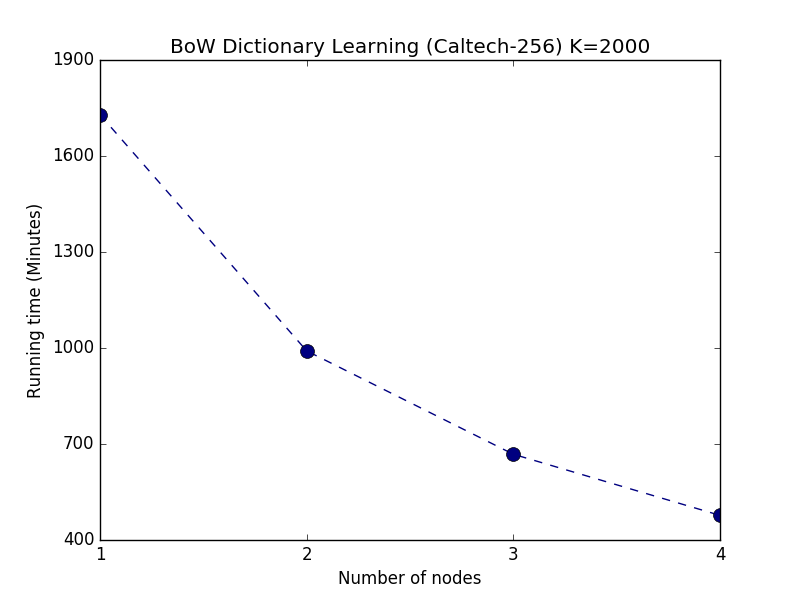
\includegraphics[width=0.66\textwidth]{bow_running_time}
  \caption{BoW字典学习计算时间}
  \label{fig:bow-running-time}
\end{figure}

在图\ref{fig:bow-running-time}可以看到BoW字典学习的计算时间。
这里计算时间单元使用分钟,SIFT抽取实验计算时间单元使用了秒。
从实验结果可以看出来,BoW词典学习支持横向扩展,增加计算节点
能按照在\ref{eq:running-time}定义的公式线性减少运行时间。
我们认为词典学习的Disk IO开销比抽SIFT特征少,另外迭代的时候
使用Spark内部缓存数据集。

\section{内存缓存性能对比实验}
\label{sec:memory-cache-experiment}
这个实验的目标是了解到CloudVision云平台的Alluxio内存缓存带来的性能。通过执行每个CloudVision机器视觉库的应用两次,
第一次输入和输出都保存到Alluxio内存缓存,第二次输入和输出都保存在集群外的Swift,这样对比每个应用的计算时间。
我们预测机器视觉库里的读写和计算比率大的应用能看到性能提高。
实验也使用了Caltech-256的数据集,里面
有30607图片和256个类别,总体数据大小是1.2GB。

缓存对比实验分析视觉库的五个应用:SIFT特征抽取(SIFT),BoW字典学习(BoW.L),SIFT转换BoW图像表示(BoW.A),
分类器训练(Class.L),分类器分类(Class.P)。每个应用跑两次对比使用Alluxio内存换春和没有用Alluxio的
计算时间。
实验使用4台计算节点处理集群,
每台计算服务器使用m1.large的配置,8 x 2.4Ghz vCPU,16GB内存,160GB本地硬盘。所有虚拟机共享一个
1Gbps私有网络。

\begin{figure}[h]
  \centering
    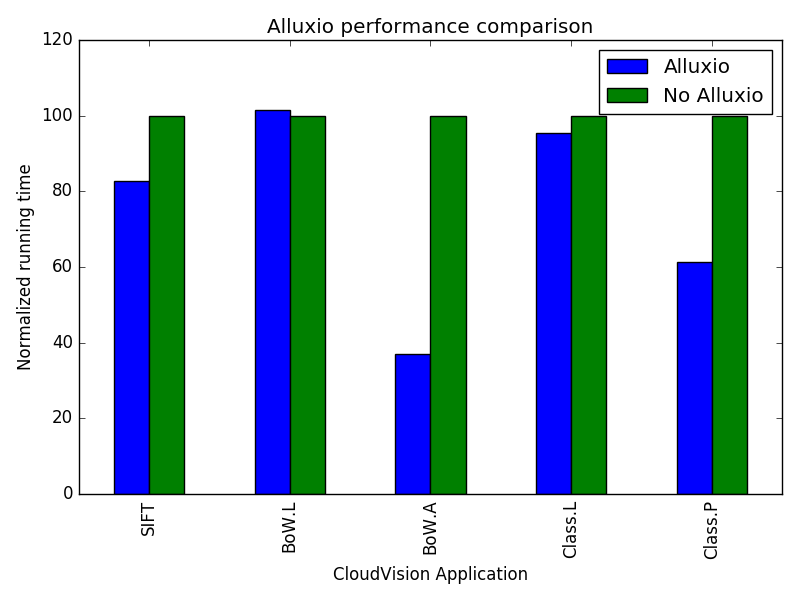
\includegraphics[width=0.66\textwidth]{alluxio_comparison}
  \caption{Alluxio跟没有Alluxio的性能对比}
  \label{fig:alluxio-comparison}
\end{figure}

在图\ref{fig:alluxio-comparison}可以看到Alluxio和没有Alluxio的性能对比,每个应用的计算时间
是表示Alluxio和没有Alluxio计算时间的比率。第一个应用SIFT特征抽(SIFT),使用Alluxio可以提高性能,
但是提高没有预测到的提高多,在分析节点的状态发现大部分时间在于CPU计算,所以读写只是应用
的一个小部分,因此用Alluxio能提高系能到17\%左右。第二个应用从SIFT特征描述子学习BoW的词典(BoW.L),
这个应用没有提高性能,其实计算时间还更高,原因是因为迭代算法主要花时间在计算,读写时间微不足道。
第三个应用用词典转换SIFT特征描述子到BoW图像表示(BoW.A),这里的性能提高很明显,
用Alluxio能提高性能63\%左右,我们认为原因是读写和计算比率高。第四个应用使用BoW图像表示和数据集标签
训练分类器,用Alluxio能提高性能6\%左右,我们认为原因是读写和计算时间比率低,应用大部分时候在算Gradient Descent。
第五个应用使用训练的分类器,分类数据集的测试集,用Alluxio能提高性能39\%左右,
原因是分类计算要求不高,因此读写和计算比率相对高。
